\documentclass{UoNMCHA}
\usepackage[authoryear]{natbib}
\usepackage{array,booktabs} % For nice tables
\usepackage{amsmath,amsfonts,amssymb} % For nice maths
\usepackage{color}
\usepackage{multicol}
\usepackage{enumerate}
\usepackage{listings}
\usepackage{subfig}
\usepackage{hyperref}
\usepackage[parfill]{parskip}   % For replacing paragraph indenting with a newline instead
\newif\ifcomment
\commenttrue
\commentfalse
% Number equations per section
\numberwithin{equation}{section}

\hypersetup{
%    bookmarks=true,         % show bookmarks bar?
%    unicode=false,          % non-Latin characters in AcrobatÕs bookmarks
%    pdftoolbar=true,        % show AcrobatÕs toolbar?
%    pdfmenubar=true,        % show AcrobatÕs menu?
%    pdffitwindow=false,     % window fit to page when opened
%    pdfstartview={FitH},    % fits the width of the page to the window
%    pdftitle={My title},    % title
%    pdfauthor={Author},     % author
%    pdfsubject={Subject},   % subject of the document
%    pdfcreator={Creator},   % creator of the document
%    pdfproducer={Producer}, % producer of the document
%    pdfkeywords={keyword1} {key2} {key3}, % list of keywords
%    pdfnewwindow=true,      % links in new window
    colorlinks=true,       % false: boxed links; true: colored links
    linkcolor=blue,          % color of internal links
    citecolor=blue,        % color of links to bibliography
%    filecolor=magenta,      % color of file links
    urlcolor=blue           % color of external links
}

\definecolor{light-gray}{gray}{0.95}
\definecolor{myblue}{RGB}{20,105,176}
\definecolor{myorange}{RGB}{255,140,0}
\definecolor{mygrey}{RGB}{64,64,64}
\definecolor{MATLABKeyword}{rgb}{0,0,1}
\definecolor{MATLABComment}{rgb}{0.1328125,0.54296875,0.1328125}
\definecolor{MATLABString}{rgb}{0.625,0.125,0.9375}

\lstset{language=Matlab,
    basicstyle=\small\ttfamily,
    keywordstyle=\color{MATLABKeyword},
    %identifierstyle=,
    commentstyle=\color{MATLABComment},
    stringstyle=\color{MATLABString},
    numberstyle=\tiny,
    %numbers=left,
    basewidth=0.5em}
\lstset{
language=C,
numbers=none,
xleftmargin=1cm,
frame=tblr,
classoffset=0,
morekeywords={LED_BUILTIN,HIGH,LOW,OUTPUT,INPUT,INPUT_PULLUP},keywordstyle=\color{myblue},
classoffset=1,
morekeywords={r0,r1,r2,r3,r4,r5,r6,r7,r8,r9,r10,r11,r12,r13,r14,r15},keywordstyle=\color{myblue},
classoffset=2,
morekeywords={ldr,srt,sub,cmp,it,bgt,b,str,ubfx,ldrb,lsl},	keywordstyle=\color{myorange},
classoffset=0,
commentstyle=\color{MATLABComment},
breaklines=true,
postbreak=\space //...
}

\firstpage{1}    % Set page number for first page
\UoNMCHAreportNo{ELEC1710  } %Report number
\UoNMCHAyear{ }   % Year
\shorttitle{ELEC1710 - Lab 5} %For odd pages
%%%%%%%%%%%%%%%%%%%%%%%%%%%%%%%%%%%%%%%%%%%%%%%%%%%%
\begin{document}
\title{Lab 5:\\ Fundamentals of Assembly Language Part 1:\\ Data Movement \\ \ \\
{\small ELEC1710  \\ 
}}
%\author[UoNMCHA]{Student Name}
%\address[UoNMCHA]{
%Student of Mechatronics Engineering,\\
%The University of Newcastle, Callaghan, NSW 2308, AUSTRALIA \\
%Student Number: 3...... \\
%E-mail: \href{mailto:First.Last@uon.edu.au}{\textsf{First.Last@uon.edu.au}}}
%%%%%%%%%%%%%%%%%%%%%%%%%%%%%%%%%%%
\maketitle
\onecolumn

\vspace{-5mm}

\section{Introduction}

This lab teaches the basics of data movement in ARM Thumb assembly. The task is to implement a look up table (LUT) which emulates a combinational logic circuit or ROM device in software.

In this case we will be emulating the  CD74HC4511 chip used in Lab 2 and so the LUT will contain 7-segment decoder data. However, here we will support all digits 0-9, A-F allowing a full hexadecimal display to be built.

\section{Program Algorithm}\label{sec:algo}

The program will be reading the 4 least significant bits of \texttt{GPIOA} and using these to address a LUT with 16 entries. Each LUT entry will be 8-bits (1 byte) wide. The data read from the LUT will be written to \texttt{GPIOB} pins 3-9 (inclusive) which can be connected to a 7-segment display. The Lookup table is provided for you. You will need to write instructions to read from GPIOA, decied which entry of the table is required, and write the corresponding table data to GPIOB.  Listing 1 shows pseudo-code for the program which is required to be translated into ARM assembly.

\begin{lstlisting}[
caption = LUT Algorithm,
label = lst:algo
]

LOOP Forever
BEGIN
    Load GPIOA port pins A3->A0 into a variable A.
    Load into X the 8-bit data which exists in LUT at line A.
    Output X to GPIOB pins 3 to 9.  // this will require a shift of the data in X so that the correct 7 bits from the table align with the correct pins.
END
\end{lstlisting}

\section{Assembly Reference}\label{sec:asm}

You will find the following instructions useful in this lab:

\subsection{Load: \texttt{ldr} and \texttt{ldrb}}

The \texttt{ldr} instruction copies data from memory (RAM, program data, GPIO pins, etc) to a CPU register. In this lab \texttt{ldr} will be used to read \texttt{GPIOA\_IDR} (GPIOA input data register) while \texttt{ldrb} is used to read bytes from a LUT located in flash memory.

Note that the registers and memory addresses are 32 bits and memory addresses specify a byte's location. The \texttt{ldr} instruction loads 4 bytes (32 bits), starting from the specified address and finishing at the address + 3. The \texttt{ldrb} instruction only loads 1 byte (8 bits) and fills the remaining 3 bytes of the destination register with zeros.

\textbf{Important:} the look-up-table must be \textit{word-aligned} (ie: start on an address which is a multiple of 4) or loading a 32-bit word from the LUT will result in an \textit{exception} which causes the CPU to jump to the \textit{default exception handler} and loop forever (ie: the CPU crashes and needs to be rebooted).

The data alignment is achieved with the assembler directive \texttt{.align 4}.

\begin{lstlisting}[
caption = Loading a register with a constant using \texttt{ldr}.,
label = 
]
ldr r3, =0x12345678
\end{lstlisting}

\begin{lstlisting}[
caption = Loading data from \texttt{GPIOA} using \texttt{ldr}.,
label = 
]
ldr r0, =GPIOA_IDR  // This constant needs to be defined in the code
ldr r1, [r0]        // Load the data at address GPIOA_IDR into r1
\end{lstlisting}

\begin{lstlisting}[
caption = Loading a register with an address from code memory using \texttt{ldr}.,
label = 
]
ldr r3, =LUT

.align 4
LUT:
    .byte 0x01
    .byte 0xFF
    .byte 0x34
\end{lstlisting}

\begin{lstlisting}[
caption = Loading a register with a byte code memory using \texttt{ldr}.,
label = 
]
ldr r3, =LUT
ldrb r4, [r3]    // Loads 0x01 into r4 from LUT

.align 4
LUT:
    .byte 0x01
    .byte 0xFF
    .byte 0x34
\end{lstlisting}

\begin{lstlisting}[
caption = Loading a register with a byte from code memory \texttt{ldr} with a constant offset.,
label = 
]
ldr r3, =LUT
ldrb r5, [r3, #2] // Loads 0x34 from LUT+2 into r5

.align 4
LUT:
    .byte 0x01
    .byte 0xFF
    .byte 0x34
\end{lstlisting}

\begin{lstlisting}[
caption = Loading a register with a byte from code memory \texttt{ldr} with a register offset.,
label = 
]
ldr r3, =LUT
ldr r2 = 0x01
ldrb r5, [r3, r2] // Loads 0xFF from LUT+1 into r5

.align 4
LUT:
    .byte 0x01
    .byte 0xFF
    .byte 0x34
\end{lstlisting}

\subsection{Store: \texttt{str}}

The \texttt{str} (store) instruction moves data from registers to a memory address. In the context of this lab it will be used to write data to \texttt{GPIOB}.

It has several forms however the syntax required for this lab is:

\texttt{str Rt, [Rn]    // Copy the data from Rt into the address in Rn}

Example:

\begin{lstlisting}[
caption = Store example.,
label = 
]
ldr r0, =GPIOB_ODR
ldr r1, =0x0
str r1, [r0]    // Move the value 0x0 to GPIOB_ODR
\end{lstlisting}


\subsection{Unsigned Bit Field Extract: \texttt{ubfx}}

The \texttt{ubfx} instruction performs an \textit{unsigned bit field extract} operation. This involves copying a given set of bits within a \textit{word} (32-bit value) to to least significant bits of a destination. The syntax is:

\texttt{ubfx Rd, Rn, \#lsb, \#width}

It moves bits from \texttt{Rn} into \texttt{Rd}, starting at bit \texttt{\#lsb} and ending at bit \texttt{\#lsb+\#width-1}. Note that bits are numbered from 0 to 31. For example:

\begin{lstlisting}[
caption = Extracting bits using ubfx.,
label = 
]
ldr r3, =0x12345678
ubfx r1, r3, #4, #4   // After execution r1 would contain the value 0x07
\end{lstlisting}

\subsection{Logical Shift Left: \texttt{lsl}}

A logical shift left moves each bit in a word one place to the left. The least significant bit is filled in with a \texttt{0} and the most significant bit is lost. \textbf{Fun fact:} This is the equivalent of multiplying by 2.

The syntax required for this lab is:

\texttt{lsl Rd, Rm, \#n}

This instruction takes the data in \texttt{Rm}, shifts it to the left by \texttt{\#n} bits and stores the result in \texttt{Rd}. This will be using for shifting a byte read from the LUT into the correct bit position for writing to \texttt{GPIOB}.

Example:

\begin{lstlisting}[
caption = Logical shift left example.,
label = 
]
ldr r0, =0x37
lsl r1, r0, #5  // After execution r1 would contain the value 0x6E0

\end{lstlisting}


\section{Hardware Configuration}

\subsection{Hardware Requirements}

\begin{itemize}
    \item Breadboard
    \item STM32F103C8T6 development board
    \item 4x Tactile push button switches
    \item 4x 10k~$\Omega$ resistors
    \item Various jumper cables
    \item Saleae logic analyser
    \item (Optional) 7x 330~$\Omega$ resistors
    \item (Optional) 1x 7-segment display
\end{itemize}

\subsection{Hardware assembly}

Perform the following construction steps:

\begin{enumerate}
    \item Ensure that the STM32 board is plugged in at one end of the breadboard with the ST-Link debug connections mounted at the edge of the breadboard.
    \item Confirm that the ST-Link debugger is connected correctly. See Lab 4 for connection details.
    \item Connect the ``V3'' pin of the STM32 board to the breadboard's Vcc rail. With the debug port pins facing up the V3 pin is located on the lower left of the board.
    \item Insert 4 push button switches and their associated pull-down resistors to create a source of a 4-bit number. See labs 1 and 2 for details regarding the push buttons.
    \item Connect each push button's output to port pins A3, A2, A1 and A0. Note that the left most push button should be the MSB and connect to A3.
    \item Connect 7 test leads from the Saleae analyser to \texttt{GPIOB} pins \texttt{B3} to \texttt{B9}.
    \item (Optional) You may wish to skip this step until the software has been written and confirmed working with the Saleae analyser.
    
    Connect the 7-segment display to the STM32 via 330~$\Omega$ resistors. \textbf{NB:} The display will be dim but using 330~$\Omega$ resistors could exceed the STM32's maximum current rating.
    
    Port pins B3, B4,..., B9 drive segments a, b,..., g respectively. User jumper cables as necessary.
    

\end{enumerate}

\section{Programming}

\subsection{Template Code}

Listing \ref{lst:code} is a template for this lab. It contains the LUT data required for driving a 7-segment display.

\begin{lstlisting}[
caption = Code listing for \texttt{sseglut.s}.,
label = lst:code
]
  .syntax unified
  .cpu cortex-m3
  .thumb
  .global sseglut

.equ    GPIOA_IDR, 0x40010808
.equ	GPIOB_ODR, 0x40010C0C

sseglut:
            // Write your code here
            // Read GPIOA_IDR
            // Extract bits required
            // Get data from LUT
            // Shift data to the correct bits
            // Write data to GPIOB_ODR
        b sseglut   // Jump back to sseglut, repeat forever
            
.align 4
ssegdata:   // The LUT
    .byte 0x3F  // 0
    .byte 0x06  // 1
    .byte 0x5B  // 2
    .byte 0x4F  // 3
    .byte 0x66  // 4
    .byte 0x6D  // 5
    .byte 0x7D  // 6
    .byte 0x07  // 7
    .byte 0x7F  // 8
    .byte 0x67  // 9
    .byte 0x77  // A
    .byte 0x7C  // B
    .byte 0x29  // C
    .byte 0x5E  // D
    .byte 0x79  // E
    .byte 0x71  // F
\end{lstlisting}

\subsection{Programming Setup}

A template for this lab is located under the Lab 4 folder on Blackboard. The code contains a \texttt{main.c} file which can, with minimal modification, be used to call any of several assembly \texttt{.s} files.

To perform this lab uncomment line 42 of \texttt{main.c} so it reads ``\texttt{sseglut();}''. This will cause the program to jump to the \texttt{sseglut:} label inside \texttt{sseglut.s}.

\subsection{Programming Task}
Using the instruction reference data in Section \ref{sec:asm} implement the algorithm in Listing \ref{lst:algo} using Thumb assembly inside \texttt{sseglut.s}. Confirm that your code works by observing the state of the appropriate \texttt{GPIOB} pins with the Saleae analyser as you input different binary numbers with the push buttons.

\subsection{Delay Measurement}

Use the Saleae analyser to measure the delay between changing the input on \texttt{GPIOA} and the corresponding bit pattern appearing on \texttt{GPIOB}. Compare this to the delay seen when using the CD74HC4511 chip.


\subsection{Debugging}

One of the table entries is incorrect (ie: the wrong, or insufficient, segments are illuminated). Find and correct this error.

\subsection{Program Memory Size}

Project part C will have some marks allocated for optimising code size. Measure the code size (in bytes) of all instructions between the \texttt{sseglut} and \texttt{ssegdata} labels. Do this by putting the debugger into ``single instruction stepping mode'', Figure \ref{fig:step}, to bring up the disassembly view and obtaining the memory addresses of the first and last instructions in the \texttt{sseglut} section, Figure \ref{fig:size}. You may use an online calculator to perform the hexadecimal subtraction. Note that you need to use the first address of the \texttt{ssegdata} section to include the size of the last instruction in \texttt{sseglut}.

\begin{figure}[h]
\makebox[\textwidth][c]{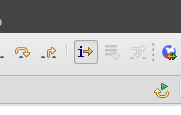
\includegraphics[width=0.4\textwidth]{instruction.png}}
\caption{Click the ``\texttt{i}'' icon to enable single instruction stepping mode and enable the disassembly view.}\label{fig:step}
\end{figure}

\begin{figure}[h]
\makebox[\textwidth][c]{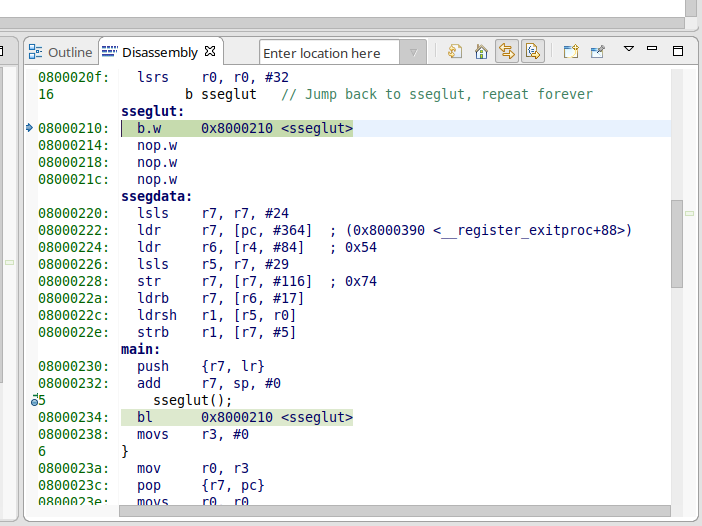
\includegraphics[width=0.7\textwidth]{asm.png}}
\caption{Dissasembly view with memory addresses for each instruction.}\label{fig:size}
\end{figure}


\end{document}